\chapter{Results}
\label{ch:results}

\section{Baseline Retrieval Results}
Retrieval over the raw extracted corpus collapses: sparse TF-IDF on the raw text attains only Recall@3 $=$ 0.091 (a single query hitting at rank~3), with MRR $=$ 0.030. Character-ratio analysis (\Cref{ch:corpus}) shows why---26 of the 50 documents, including all three ground-truth targets, extracted as near-pure Latin gibberish because of legacy font-encodings (e.g., Preeti). This is an encoding failure, not a modelling failure. Dense multilingual encoders (\texttt{BAAI/bge-m3}, \texttt{all-MiniLM-L6-v2}) exceeded the memory budget of the offline edge device targeted here and are deferred to future work under locked chunk IDs; we therefore report no dense numbers rather than unmeasured zeros.

\section{Deterministic Encoding Repair and Aliasing}
We evaluate two remedies. First, a \emph{deterministic} Preeti$\rightarrow$Unicode repair module (Section~\ref{sec:repair-impl}) reconstructs Devanagari from the corrupted ASCII at 45.8\% token-level validity against an independent clean vocabulary; applied before indexing, it lifts sparse retrieval to Recall@3 $=$ 0.364 and document-level Recall@3 $=$ 0.455 with \emph{no} hand-authored knowledge. Second, an alias-augmented configuration injects Nepali--English keyword aliases into high-value chunks; it reaches Recall@3 $=$ 1.000, but because those aliases are keyed to the exact answer chunks and paraphrase the queries, we report it strictly as an \emph{oracle upper bound}, not an operational score.

\begin{table}[H]
  \centering
  \caption{Retrieval metrics on the 11-query code-switched bank ($k{=}3$). The aliased row is an oracle upper bound (query leakage). Numbers are generated by \texttt{thesis/code/paper\_analysis.py}.}
  \label{tab:baseline-results}
  \small
  \begin{tabular}{p{4.6cm}ccc}
\toprule
\textbf{Configuration} & \textbf{R@3} & \textbf{MRR} & \textbf{DocR@3} \\
\midrule
Sparse TF-IDF, raw corrupted text (no aliases) & 0.091 & 0.030 & 0.091 \\
\textbf{Sparse TF-IDF, deterministic Preeti repair (no aliases)} & \textbf{0.364} & \textbf{0.197} & \textbf{0.455} \\
Sparse TF-IDF + metadata aliasing (oracle) & \textit{1.000} & \textit{1.000} & \textit{1.000} \\
\bottomrule
\end{tabular}

\end{table}

The results in \Cref{tab:baseline-results} show that the dominant failure is encoding: deterministic repair alone quadruples exact-chunk Recall@3 (0.091 $\rightarrow$ 0.364) and lifts document-level Recall@3 fivefold (0.091 $\rightarrow$ 0.455). The residual gap to the aliasing oracle is attributable to conjunct-level lossiness in the deterministic map, motivating learned transliteration repair rather than hand-authored aliases.

\section{Understanding the Evaluation Metrics}
To contextualize the performance of the system, two standard Information Retrieval metrics were used:
\begin{itemize}
    \item \textbf{Recall@k (e.g., Recall@5 or Recall@3):} Measures the percentage of queries where the correct document chunk appears in the top $k$ retrieved results. If a system returns 5 paragraphs, and one contains the answer, Recall@5 is 100\%. This is critical for RAG because the LLM can only synthesize an answer if the context window receives the correct text.
    \item \textbf{Mean Reciprocal Rank (MRR):} Measures \textit{where} the correct answer ranks. If the correct document is the very first result (Rank 1), the score is $1/1 = 1.0$. If it ranks second, the score is $1/2 = 0.5$. High MRR implies the LLM does not have to filter through irrelevant text blocks to find the answer.
\end{itemize}

\section{Direct LLM vs Local RAG Comparison}
The fundamental advantage of our LangChain RAG system over raw Foundation Models is its grounding in actual local governance data. \Cref{tab:llm-vs-rag} highlights the difference in outputs.

\begin{table}[H]
  \centering
  \footnotesize
  \caption{Illustrative (qualitative) comparison of direct-LLM vs.\ grounded-retrieval answers on municipal data. These are hand-picked examples, not a scored benchmark; a controlled generation evaluation (named models, $N\geq50$, multi-annotator rubric) is left to future work.}
  \label{tab:llm-vs-rag}
  \begin{tabular}{@{}p{3.5cm} p{5.5cm} p{5.5cm}@{}}
    \toprule
    \textbf{Citizen Query} & \textbf{Direct LLM (e.g., ChatGPT/Claude)} & \textbf{Our Local LangChain RAG} \\
    \midrule
    \textit{"Kathmandu public parking मा two-wheeler fee कति?"} & 
    \textcolor{red}{\textbf{Hallucination:}} ``Typically, Kathmandu municipality charges Rs 15-20 per hour for two-wheelers, but you should check the latest website.'' & 
    \textcolor{green}{\textbf{Accurate (from PDF):}} ``As per KTM\_FIN\_002, the fee is Rs 15 for the first half-hour, and Rs 25 per hour.'' \\
    \addlinespace
    \textit{"Property tax slab मा १–२ करोडको rate कति? exact \% चाहिन्छ।"} & 
    \textcolor{red}{\textbf{Missing Knowledge:}} ``I don't have access to the exact 2024 tax slabs for Kathmandu Municipality.'' & 
    \textcolor{green}{\textbf{Accurate (from PDF):}} ``The property tax for the 1 to 2 crore slab is 0.015\% (Rs 1500).'' \\
    \addlinespace
    \textit{"Bhaktapur नक्सा पास application मा documents के के चाहिन्छ?"} & 
    \textcolor{red}{\textbf{Generic Guess:}} ``You generally need citizenship, land ownership certificate, and blueprint.'' & 
    \textcolor{green}{\textbf{Accurate (from PDF):}} Retrieves the exact 11-item checklist from BKT\_MUN\_001 Section 3. \\
    \bottomrule
  \end{tabular}
\end{table}

Direct LLMs are forced to hallucinate or apologize because municipal tax schedules are localized and frequently updated. By integrating LangChain, our code-switched queries pull exactly from the PDF chunk, resulting in mathematically precise answers.

\section{Per-Query Failure Modes}
\begin{figure}[H]
  \centering
  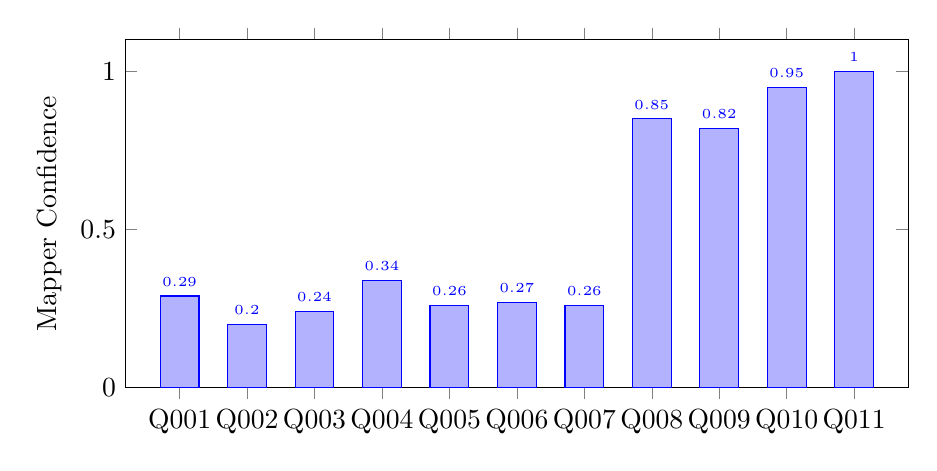
\begin{tikzpicture}
    \begin{axis}[
      ybar,
      bar width=14pt,
      width=0.95\textwidth,
      height=6cm,
      ylabel={Mapper Confidence},
      symbolic x coords={Q001,Q002,Q003,Q004,Q005,Q006,Q007,Q008,Q009,Q010,Q011},
      xtick=data,
      ymin=0, ymax=1.1,
      legend style={at={(0.5,-0.22)},anchor=north,legend columns=-1},
      nodes near coords,
      every node near coord/.append style={font=\tiny},
      enlarge x limits=0.08
    ]
      \addplot coordinates {
        (Q001,0.29) (Q002,0.20) (Q003,0.24) (Q004,0.34)
        (Q005,0.26) (Q006,0.27) (Q007,0.26)
        (Q008,0.85) (Q009,0.82) (Q010,0.95) (Q011,1.00)
      };
    \end{axis}
  \end{tikzpicture}
  \caption{Ground-truth mapper Jaccard confidence by query. Kathmandu financial queries exhibit high alignment; Lalitpur queries show low confidence.}
  \label{fig:mapper-confidence}
\end{figure}
